
%(BEGIN_QUESTION)
% Copyright 2013, Tony R. Kuphaldt, released under the Creative Commons Attribution License (v 1.0)
% This means you may do almost anything with this work of mine, so long as you give me proper credit

Sketch connecting wires allowing channel {\tt IN 4} on the data acquisition (DAQ) module to sense the full speed range of the tachogenerator (``tach'') which outputs 0 to 10 volts over a rotational speed range of 0 to 1500 RPM (revolutions per minute).  Feel free to add any additional components you deem necessary to this circuit!

\vskip 50pt

$$\includegraphics[width=15.5cm]{i03471x01.eps}$$

\underbar{file i03471}
%(END_QUESTION)





%(BEGIN_ANSWER)

A voltage divider circuit will be necessary to reduce the tach's voltage to a range the DAQ can sense.

$$\includegraphics[width=15.5cm]{i03471x02.eps}$$

%(END_ANSWER)





%(BEGIN_NOTES)

{\bf This question is intended for exams only and not worksheets!}.

%(END_NOTES)

